%% -*- Lecture -*-

\documentclass[11pt,aspectratio=169]{beamer}

\usepackage{rcstalk}
\usetheme{rcstheme}

\usepackage{tikz}
\usetikzlibrary{shapes,arrows,shadows,positioning,patterns,matrix,calc}
\usepackage{pgf}

\subtitle{Debugging}
\topic{Debugging Traps and Pitfalls}

\begin{document}

\maketitle

\begin{slide}{Finding and Fixing Bugs}
\itms{
    \item "An ounce of prevention is worth a pound of cure." - Benjamin 
	Franklin
    \gap
    \item Preventative Approaches:
    \ittms{
	\item Compiler Tools
	\item Defensive Programming
	\item Static/Dynamic Analysis
	\item Runtime Checkers
    }
    \gap
    \item Debugging Approaches:
    \ittms{
	\item Debuggers
	\item Log Debugging
    }
}
\end{slide}

\section{Preventative Approaches}

\begin{slide}{Compiler Tools}
\itms{
    \item Compiler's can help you avoid bugs:
    \gap
    \item Enable warning and convert warnings into errors.
    \item \code{CFLAGS=-Wall -Werror}
    \gap
    \item Don't ignore warnings particularly:
    \ittms{
	\item Uninitialized variables
	\item Undefined behavior
    }
    \gap
    \item Sometimes \code{-Wall} enables some benign warnings like unused 
	arguments
}
\end{slide}

\begin{slide}{Use the Language/Compiler To Detect Bugs}
\itms{
    \item Don't initialize variables until you need to
    \ittms{
	\item Allows the compiler to analyze your code
	\item Show you cases were you may not intend to use a default value
    }
}
\begin{columns}
\column{0.5\textwidth}
\begin{ccode}
void foo() {
    int status = 0;
    ...
    if (...) {
	status = 1;
	return status;
    }

    return status;
}
\end{ccode}
\column{0.5\textwidth}
\begin{ccode}
void foo() {
    int status;
    ...
    if (...) {
	status = 1;
	return status;
    }

    /*
     * Warning: use of unassigned
     * local variable.
     */
    return status;
}
\end{ccode}
\end{columns}
\end{slide}

\begin{slide}{Use the Language/Compiler To Detect Bugs}
\itms{
    \item Always check return values
    \ittms{
    \item Ignoring return values often make debugging hard
    \item Happens often to students in our assignments
    }
    \gap
    \item Prevent developers from ignoring important results
    \ittms{
    \item Example: \code{int pthread_mutex_trylock(...) __attribute__((warn_unused_result));}
    \item No correct way to use trylock without checking the return value
    }
    \gap
    \item Disable implicit casting
    \ittms{
    \item Force you to explicitly cast types and think about type safety
    }
}
\end{slide}

\begin{slide}{Defensive Programming: Asserts}
\itms{
    \item Use \code{assert} to check any pre-/post-conditions
    \ittms{
	\item If you aren't checking if an input is valid
	\item Then your assuming a condition
    }
    \gap
    \item You can also insert compile time checks \code{static_assert}
}
\begin{ccode}
void foo(...) {
    assert(precondition ...);

    ...

    assert(postcondition ...);

    return status;
}
\end{ccode}
\end{slide}

\begin{slide}{Defensive Programming}
\itms{
    \item Avoid bool, define flags that aren't easy to mix up
    \ittms{
    \item Worse: inverting the flag in software layers
    \item Use \code{enum} to define explicit flags
    }
    \gap
    \item Use \code{enum} for switch-case statements
    \ittms{
    \item Avoid default case if possible
    \item Compiler warns of missing enum cases
    }
    \gap
    \item Avoid confusing APIs
    \ittms{
    \item Example: \man{strncpy} vs. \man{strlcpy} and \man{strncat} vs.  
	\man{strlcat}
    \item \code{strncpy} doesn't null terminate the string when the buffer is too small!
    }
}
\end{slide}

\begin{slide}{Static Analysis}
\centering
    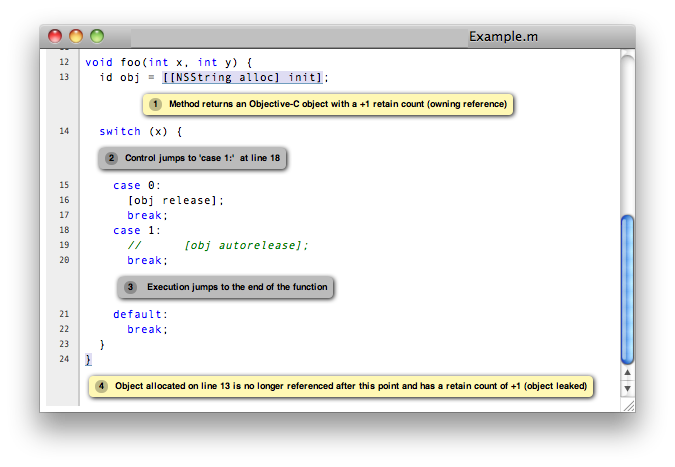
\includegraphics[scale=0.35]{analyzer_html.png}
\itms{
    \item Clang Static Analyzer
    \item See: \cref{readings/klee.pdf}{[KLEE]}, 
	\cref{readings/coverity.pdf}{[Coverity]}
}
\end{slide}

\begin{slide}{Runtime Checkers}
\begin{ccode}
#include <pthread.h>
int Global;
void *Thread1(void *x) {
  Global = 42;
  return x;
}
int main() {
  pthread_t t;
  pthread_create(&t, NULL, Thread1, NULL);
  Global = 43;
  pthread_join(t, NULL);
  return Global;
}
\end{ccode}
\itms{
    \item ThreadSanitizer, AddressSanitizer, ...
    \item See: \cref{readings/eraser.pdf}{[Eraser]}, 
	\cref{readings/threadsan.pdf}{[ThreadSanitizer]}
}
\end{slide}
\begin{slide}{Runtime Checkers: ThreadSanitizer}
\begin{verbatim}
% ./a.out
WARNING: ThreadSanitizer: data race (pid=19219)
  Write of size 4 at 0x7fcf47b21bc0 by thread T1:
    #0 Thread1 tiny_race.c:4 (exe+0x00000000a360)

  Previous write of size 4 at 0x7fcf47b21bc0 by main thread:
    #0 main tiny_race.c:10 (exe+0x00000000a3b4)

  Thread T1 (running) created at:
    #0 pthread_create tsan_interceptors.cc:705 (exe+0x00000000c790)
    #1 main tiny_race.c:9 (exe+0x00000000a3a4)
\end{verbatim}
\itms{
    \item ThreadSanitizer, AddressSanitizer, ...
    \item See: \cref{readings/eraser.pdf}{[Eraser]}, 
	\cref{readings/threadsan.pdf}{[ThreadSanitizer]}
}
\end{slide}


\pgfdeclarelayer{background}
\pgfdeclarelayer{foreground}
\pgfsetlayers{background,main,foreground}
\tikzstyle{stk}=[draw, fill=white, text width=9em, text centered, minimum 
height=14.75em]
\tikzstyle{sstk}=[draw, fill=white, text width=9em, text centered, minimum 
height=1.5em]
\tikzstyle{mstk}=[draw, fill=white, text width=9em, text centered, minimum 
height=4em]
\tikzstyle{lstk}=[draw, fill=white, text width=9em, text centered, minimum 
height=6em]
\tikzstyle{lbl}=[align=center]

\section{Debugging Approaches}

\begin{frame}{Debuggers}
\itms{
    \item Debuggers are great!
    \gap
    \item Some classes push debuggers because it's an important skill
    \gap
    \item Throughout VMware and Ph.D.:
    \ittms{
    \item Used debuggers to inspect crashes (rarely)
    \item Used log debugging for everything else
    \item Requires displined use of logging throughout the code
    }
}
\end{frame}

\begin{frame}{Effective Logging}
\itms{
\item Basics
    \ittms{
    \item Log major operations
    \item Turn on/off logging per subsystem
    \item Compile out unnecessary logs
    \item Timestamp every message
    }
    \gap
    \item Every log message should print a unique identifier (e.g., task/object)
    \ittms{
    \item Use \code{grep} to quickly filter relevant events
    }
    \gap
    \item Dump state on a crash: register signal handlers
}
\end{frame}

\begin{frame}{Log Debugging Pitfalls}
\itms{
\item Three examples of what can go wrong...
\gap
\item Non-maskable Interrupts, Machine Check Exceptions, etc.
\item Logging, Locks and Heisenbugs
}
\end{frame}


%\begin{frame}{Log Debugging Pitfalls: NMIs}
%\itms{
%    \item What can go wrong?
%}
%\begin{figure}
%\begin{tikzpicture}
%	\node (f0) [stk] {};
%	\path (f0.north) node (f1) [sstk] {{\tt \_start} frame};
%	\path (f1)+(0,-1.5em) node (f2) [sstk] {{\tt main()} frame};
%	\path (f2)+(0,-1.5em) node (f3) [sstk] {{\tt printf()} frame};
%	\path (f3)+(0,-1.5em) node (f4) [sstk] {{\tt write()} frame};
%	\path (f0.south)+(0,-1em) node (lbl) {User Stack};
%
%	\path (f0)+(10em,0) node (k0) [stk] {};
%	\path (k0.north)+(0,-1.25em) node (k1) [mstk]
%	{{\tt common\_exception}\\{\em trapframe}};
%	\path (k1)+(0,-2.75em) node (k2) [sstk] {\tt trap()};
%	\path (k2)+(0,-1.5em) node (k3) [sstk] {\tt syscall()};
%	\path (k3)+(0,-1.5em) node (k4) [sstk] {\tt sys\_write()};
%	\path (k4)+(0,-1.5em) node (k5) [sstk] {\em console driver};
%	\path (k0.south)+(0,-1em) node (lbl) {Kernel Stack};
%\end{tikzpicture}
%\end{figure}
%\end{frame}
%
%\begin{frame}{Log Debugging Pitfalls: NMIs}
%\itms{
%    \item What can go wrong? NMI arrives while holding spinlocks!
%}
%\begin{figure}
%\begin{tikzpicture}
%	\node (f0) [stk] {};
%	\path (f0.north) node (f1) [sstk] {{\tt \_start} frame};
%	\path (f1)+(0,-1.5em) node (f2) [sstk] {{\tt main()} frame};
%	\path (f2)+(0,-1.5em) node (f3) [sstk] {{\tt printf()} frame};
%	\path (f3)+(0,-1.5em) node (f4) [sstk] {{\tt write()} frame};
%	\path (f0.south)+(0,-1em) node (lbl) {User Stack};
%
%	\path (f0)+(10em,0) node (k0) [stk] {};
%	\path (k0.north)+(0,-1.25em) node (k1) [mstk]
%	{{\tt common\_exception}\\{\em trapframe}};
%	\path (k1)+(0,-2.75em) node (k2) [sstk] {\tt trap()};
%	\path (k2)+(0,-1.5em) node (k3) [sstk] {\tt syscall()};
%	\path (k3)+(0,-1.5em) node (k4) [sstk] {\tt sys\_write()};
%	\path (k4)+(0,-1.5em) node (k5) [sstk] {\em console driver};
%	\path (k5)+(0,-1.5em) node (k6) [sstk] {\em trapframe \#2};
%	\path (k6)+(0,-1.5em) node (k7) [sstk] {\tt trap()};
%	\path (k7)+(0,-1.5em) node (k8) [sstk] {\tt kprintf()};
%	\path (k0.south)+(0,-1em) node (lbl) {Kernel Stack};
%\end{tikzpicture}
%\end{figure}
%\end{frame}

\begin{frame}{Log Debugging Pitfalls: NMIs}
\itms{
    \item What can go wrong?
    \gap
    \item Logging code is fairly complex: \code{*printf}, console, and serial 
	devices
    \item Can't use Mutex locks inside of a spinlock region...
    \gap
    \item \code{kprintf} avoids locking
    \item Console and serial driver implement spinlocks per character
    \item Similar to a Mutex, but disables interrupts.
    \item Unfortunately, certain interrupts cannot be disabled
    \item Result: thread deadlocks with itself
    \gap
    \pause
    \item Bad choices: potential for deadlocks or expose potential races
    \item Similar problems can happen in complex software (e.g. with signals)
}
\end{frame}

\begin{frame}{Log Debugging Pitfalls: NMIs - Solutions}
\itms{
    \item Solutions:
    \ittms{
    \item Drop log messages if device locks held
    \item Attempt to write to device without locks
    \item Attempt to acquire locks using trylock
    \item Buffer locks in a lock-free buffer
    }
    \gap
    \pause
    \item Both result in unreliable logging
    \item Probably you want to attach a debugger
}
\end{frame}

\begin{frame}{Log Debugging Pitfalls: Locks, Logs and Heisenbugs}
\itms{
    \item Logging infrastructure uses locks!
    \gap
    \pause
    \item Logging can:
    \ittms{
	\item Serialize operations hiding data races (implicit barriers and 
	    locks)
	\item Change timing hiding data races
    }
    \gap
    \pause
    \item What can you do?
    \ittms{
	\item Reproduce bug with and without logging
	\item Look for data races
    }
}
\end{frame}

\begin{frame}{Summary}
\itms{
\item Logs can be reordered if there's buffering
\item Logging can deadlock or be dropped silently
\item Logging can hide races (it slows you down)
}
\end{frame}

%\begin{figure}
%\begin{tikzpicture}
%	\node (f0) [stk] {};
%	\path (f0.north) node (f1) [sstk] {{\tt \_start} frame};
%	\path (f1)+(0,-1.5em) node (f2) [sstk] {{\tt main()} frame};
%	\path (f0.south)+(0,-1em) node (lbl) {User Stack};
%
%	\path (f0)+(10em,0) node (k0) [stk] {};
%	\path (k0.north)+(0,-1.25em) node (k1) [mstk]
%	{{\tt common\_exception}\\{\em trapframe}};
%	\path (k1)+(0,-2.75em) node (k2) [sstk] {\tt mips\_trap()};
%	\path (k2)+(0,-1.5em) node (k3) [sstk] {\tt mainbus\_interrupt};
%	\path (k3)+(0,-1.5em) node (k4) [sstk] {\tt timer\_interrupt};
%	\path (k4)+(0,-1.5em) node (k5) [sstk] {\tt thread\_yield};
%	\path (k5)+(0,-1.5em) node (k6) [sstk] {\tt thread\_switch};
%	\path (k6)+(0,-2.75em) node (k7) [mstk] {\em switchframe};
%	\path (k0.south)+(0,-1em) node (lbl) {Kernel Stack 1};
%\end{tikzpicture}
%\end{figure}
%\end{frame}

\end{document}

